\section{Interaction Traces}
\label{app:trace}

Figure~\ref{fig:workflow} follows two requests from the frozen evaluation through the pipeline: the candidates are recorded outputs, and the gate verdicts are recomputed with the deterministic validator.

\begin{figure*}[t]
\centering
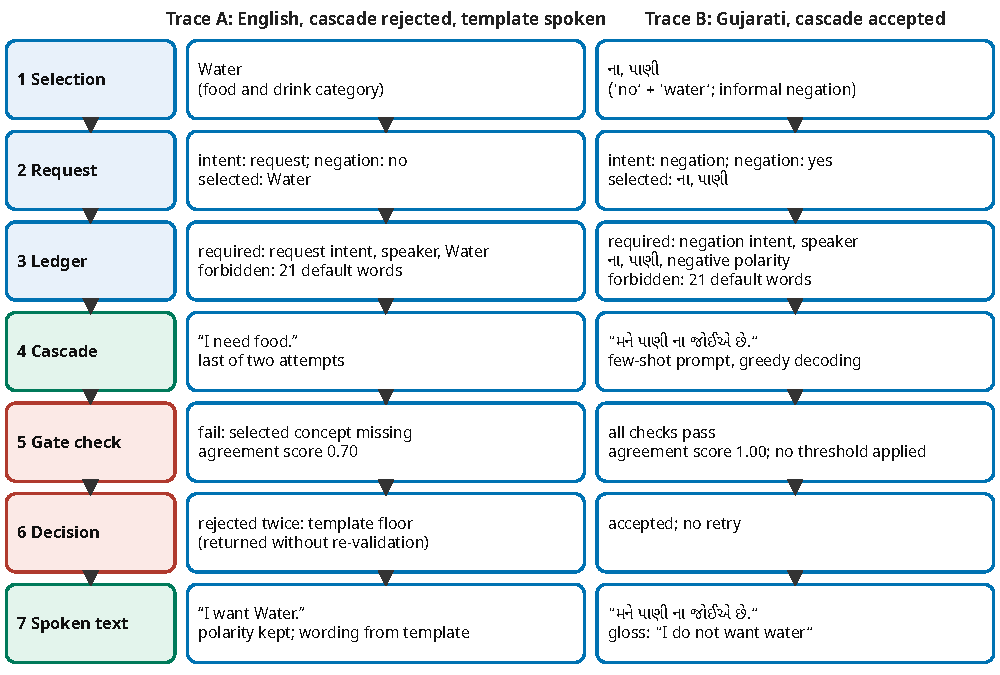
\includegraphics[width=\textwidth]{figures/workflow.pdf}
\caption{Interaction traces. Trace A: an English request whose cascade output is rejected twice and replaced by the template. Trace B: a Gujarati request whose cascade output is accepted; gloss: ``I do not want water'' (informal negation).}
\label{fig:workflow}
\end{figure*}

\section{Scorer Definitions and Scenario Families}
\label{app:scorer}
Retention is the share of required concept instances present (lexicon forms with inflection stems).
Polarity is correct when a negator is present exactly if the gold message is negated.
The act is correct when a request marker (want, need, \hi{चाहिए}, \gu{જોઈએ}, \hi{हवे}) or, for feelings, a feeling marker without a request marker is present.
A concept is \emph{added} if any other board concept or a time, meal, or venue word occurs.
An output is \emph{off-task} if it is a refusal, a third-person report (``the user\ldots''), empty, longer than 25 tokens, or contains Latin text in an Indic target.
Scenarios, lexicon, scorer, and raw outputs are in the release package; Table~\ref{tab:type} breaks success down by scenario family.
On the eight exploratory Hinglish scenarios the deployed pipeline succeeds on \CMSuccDepU{} (client) and \CMSuccDepS{} (explicit), the unconstrained prompt on \CMSuccNaive{}, and the template on \CMSuccTmplU{} and \CMSuccTmplS{}.

\begin{table}[t]
\centering\footnotesize
\setlength{\tabcolsep}{2.6pt}
\begin{tabular}{@{}lcccccc@{}}
\toprule
 & \multicolumn{3}{c}{Client payload} & \multicolumn{3}{c}{Explicit fields} \\
\cmidrule(lr){2-4}\cmidrule(l){5-7}
Scenario family ($n$) & Pre & Dep. & Tmpl & Pre & Dep. & Tmpl \\
\midrule
Food/drink request (35) & 26 & 29 & 35 & 26 & 29 & 35 \\
Refusal (\emph{No}+food) (38) & 19 & 33 & 38 & 10 & 38 & 38 \\
Feeling (30) & 3 & 4 & 5 & 18 & 22 & 30 \\
Negated feeling (32) & 2 & 1 & 0 & 2 & 13 & 24 \\
Action + object (24) & 8 & 18 & 24 & 8 & 18 & 24 \\
Help/call + person (16) & 7 & 12 & 16 & 7 & 12 & 16 \\
\midrule
All (175) & 65 & 97 & 118 & 71 & 132 & 167 \\
\bottomrule
\end{tabular}
\caption{Successful scenarios by family on the primary set. Pre: cascade before the gate; Dep.: deployed output; Tmpl: template floor.}
\label{tab:type}
\end{table}


\section{Trained Components}
\label{app:models}

Table~\ref{tab:models} lists the learned components.
Qwen2.5-0.5B-Instruct and IndicF5 are used as released.
\emph{Refiner.} The English refiner fine-tunes Flan-T5-small (76,961,152 parameters) to map selected concepts and an intent to one sentence, with 32-bit floating point, learning rate $10^{-4}$, weight decay 0.01, batch size 16 with two accumulation steps, 10 epochs (960 updates), seed 42, and one NVIDIA TITAN Xp (204\,s); the checkpoint with the lowest validation loss is kept.
Training, validation, and test hold 3,052, 384, and 384 template-generated payloads in 318, 40, and 40 disjoint groups; a fluency arm first adapts for 500 updates on 4,380 denoising pairs.
On the test payloads the fine-tuned model reaches \RefAModel{} exact match (\RefFModel{} with fluency pre-adaptation) and makes no negation error in 172 negated payloads, at a median of \RefALat{}\,ms; rules and the hybrid score \RefARules{} because references come from the same template families.

\begin{table*}[t]
\centering\footnotesize
\setlength{\tabcolsep}{3pt}
\begin{tabular}{@{}L{2.9cm}L{2.2cm}L{7.3cm}L{2.6cm}@{}}
\toprule
Component & Role in the demo & Training or adaptation & Data \\
\midrule
Qwen2.5-0.5B-Instruct (rev.\ 7ae5576) & realizer, refiner, verifier & Prompted, not fine-tuned (few-shot for HI, GU, MR) & -- \\
IndicF5 + Vocos & speech & Pretrained; zero-shot voice conditioning on a clip and its transcript & 1,417\,h, four corpora \\
HMM-1, HMM-2 & optional fallback prediction; Un-Jumble & Streamed in 500K-sentence chunks, pruned at counts 3 (4-grams) and 2 (trigrams). HMM-1: Jelinek--Mercer weights .50/.30/.15/.05. HMM-2: word and POS trigrams, exact search to 6 words, beam 64 above & English high-quality sentences, Tatoeba, Pile slices \\
Gutenberg HMM & English baseline & Bigram and trigram counts: 188,402 sentences; 63,783 bigram and 713,845 trigram states & public-domain books \\
Hindi AAC HMM & Hindi fallback & 3,867 turns, 2,171 word types (retrained on 3,078 training turns for evaluation) & Hindi dialogues \\
Suffix trie ($\infty$-gram) & primary next word & Count-based, built at start-up (\IGSent{} sentences, depth \IGDepth{}) & EN and HI dialogues \\
Flan-T5-small refiner & companion tool & Fine-tuned as described above & 3,052 template payloads \\
\bottomrule
\end{tabular}
\caption{Learned components, from the training records, run configurations, and model files in the release package. The IndicF5 corpora are Rasa, IndicTTS, LIMMITS, and IndicVoices-R.}
\label{tab:models}
\end{table*}
